\subsection{Espectroscopia Mössbauer: División de picos}

Una perspectiva diferente en el estudio de la estructura atómica local puede 
obtenerse con la técnica espectroscópica de Mössbauer, que consiste en medir 
la emisión o la absorción de rayos gamma asociada a las transiciones de niveles
de energía en el núcleo \cite{long2013}. Estos niveles de energía están 
influenciados por el entorno local, que puede cambiar o dividir estos niveles.
Esta técnica fue utilizada por Li \textit{et al.} para medir los espectros de 
Mössbauer de rayos gamma de $^{119}$Sn en estructuras amorfas de 
Li$_x$Si$_{1-y}$Sn$_y$ para $0 < x < 3.5$ y valores pequeños de $y$ \cite{li2009}.
Dadas las concentraciones bajas de estaño, los autores asumen que los átomos de Sn
ocupan los mismos sitios que los de átomos de Si en este material, haciendo que 
las conclusiones inferidas para el Sn sean equivalentes para el Si 
\cite{hatchard2005}. La señal de MB consiste en dos picos que se superponen casi 
completamente en los casos extremos de concentraciones bajas o altas de Li, 
pero están claramente separados para casos intermedios. La distancia de separación
$\Delta$ se espera que sea sensible al entorno local de los átomos de Sn. $\Delta$
alcanza un valor máximo al rededor de $1.2$ mm/s para $x \sim 1$ y decrece para 
valores mayores o menores de $x$ (ver los triángulos en la Figura \ref{fig:mossbauer}).
\begin{figure}[h!]
    \centering
    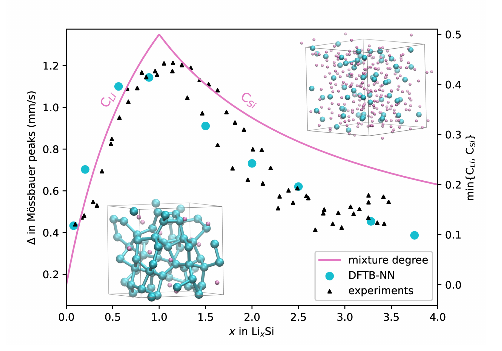
\includegraphics[width=.7\textwidth]{Silicio/prediccion/resultados/mossbauer/mossbauer.png}
    \caption{Desplazamiento entre los dos picos en los espectros de efecto 
    Mössbauer. Los triángulos que apuntan hacia arriba corresponden a dos 
    medidas de Li \text{et al.} (eje de la izquierda), la línea discontinua es la 
    predicción de la ecuación \ref{eq:mossbauer}, utilizando concentraciones 
    medias de átomos de Li y Si. Los círculos azules son las predicciones dadas 
    por la ecuación \ref{eq:mossbauer}, con $C_{\text{Li}}$ , $C_{\text{Si}}$ 
    calculados a partir de la concentración de los vecinos más cercanos (eje de 
    la derecha). Las barras de error son menores que el tamaño de los puntos.}
    \label{fig:mossbauer}
\end{figure}
Los autores sugieren que el valor máximo de $\Delta$ se obtiene cuando los átomos 
de Sn (y por analogía los de Si) están rodeados por una mezcla equimolar de Si y 
Li, y luego decrece cuando alguno de los dos tipos de átomos predomina. Con el fin 
de formular en términos cuantitativos esta idea, se define la concentración de 
átomos de Li ($C_{\text{Li}}$) y la concentración de átomos de Si 
($C_{\text{Si}}$) en términos del número de átomos de Li en la formula Li$_x$Si:
\begin{equation}\label{eq:clicsi}
    C_{\text{Li}} = \frac{x}{1+x} \hspace{2cm}y \hspace{2cm}  C_{\text{Si}} = 1 - C_{\text{Li}}.
\end{equation}
Ahora, como se observa en los datos experimentales de la Figura \ref{fig:mossbauer}
que $\Delta$ tiende a un valor constante para valores pequeños y grandes de $x$, 
se propone el siguiente \textit{ansatz} para $\Delta$:
\begin{equation}\label{eq:mossbauer}
    \Delta = a\min\left\lbrace C_{\text{Li}},C_{\text{Si}}\right\rbrace + b.
\end{equation}
Regulando los valores de $a$ y $b$ es posible ver (curva naranja discontinua en 
la Figura \ref{fig:mossbauer}) que esta dependencia simple produce la tendencia 
cualitativa del experimento. Sin embargo, la definición dada en la ecuación 
\ref{eq:clicsi} depende del contenido de Li promedio en la aleación, mientras que 
MB percibe el entorno local. Se puede buscar una mejor concordancia si se calculan 
estos valores de concentraciones de Li y Si considerando los vecinos más cercanos
de cada átomo de Si para cada estructura amorfa obtenida en las simulaciones de
dinámica molecular. Si se reemplazan estos valores locales de $C_{\text{Li}}$ y 
$C_{\text{Si}}$ en la ecuación \ref{eq:mossbauer} se obtienen los puntos azules
de la Figura \ref{fig:mossbauer}, que muestran una mejora en la concordancia 
con los experimentos.
